%% ITAT 2026 / CEUR-WS submission
\documentclass[]{ceurart}

\sloppy
\usepackage{listings}
\lstset{breaklines=true}
\usepackage{amsmath,amssymb}
\usepackage{booktabs}
\usepackage{tikz}
\usetikzlibrary{positioning, arrows.meta}

\begin{document}

\copyrightyear{2026}
\copyrightclause{Copyright for this paper by its authors.
  Use permitted under Creative Commons License Attribution 4.0
  International (CC BY 4.0).}

\conference{ITAT 2026: Information Technologies -- Applications and Theory,
  September 2026, Slovakia}

\title{Automated Conjecturing Pipeline for Graph Theory}

\tnotemark[1]
\tnotetext[1]{All code, databases, and verification scripts described here are
  reproducible from the artefacts accompanying this paper.}

\author[1]{Author One}[%
email=author.one@example.org,
]
\cormark[1]
\address[1]{Affiliation, City, Country}

\cortext[1]{Corresponding author.}

\begin{abstract}
  We report a complete, reproducible campaign to make an automated
  graph-theoretic conjecturing system that is \emph{honest by construction}.
  Starting from a TxGraffiti-style generator of linear inequalities between
  graph invariants, we add four ingredients that, together, change the
  character of the output: (i) an \emph{exact-or-blank} database that unions
  the House of Graphs invariant export, an exhaustive census of all connected
  graphs on at most nine vertices, and several special graph families
  (strongly regular, minimal Ramsey, Cayley, cages), with every unreliable
  approximate value removed; (ii) a \emph{novelty filter} of $203$ classical
  and trivial theorems closed under transitive composition and linear
  identity substitution, which decides whether a candidate is implied by known
  mathematics; (iii) an \emph{adversarial verification stage}, a permanent part
  of the pipeline, that tests every candidate against a pool of
  structure-targeted graphs (barbells, lollipops, spiders, class generators)
  built specifically to break loose database-only bounds; and (iv) an extension
  to product/ratio conjectures. We then validate a structure-seeded
  counterexample-search engine by independently rediscovering, at the published
  optimal score, the counterexample to the Aouchiche--Hansen conjecture
  $\lambda_1+\mu\ge\sqrt{n-1}+1$, and we exhaustively verify a range of open
  conjectures (Reed; recent independent-domination bounds; sixteen
  Graffiti.pc/TxGraffiti conjectures) on all connected graphs up to nine
  vertices. We further integrate the \textsc{Conjecturing} package of Larson and
  Van~Cleemput---a reference implementation of Fajtlowicz's Dalmatian
  heuristic that searches over \emph{expression trees} rather than fixed linear
  templates---so that the generator's hypothesis language extends to sums,
  products, ratios, powers, and roots of invariants, with known bounds injected
  as a \emph{theory} so that only strictly more significant statements survive.
  The central, repeatedly confirmed finding is methodological: the
  space of inequalities among classical invariants on
  standard graph collections yields known mathematics, and every apparent
  ``discovery'' the pipeline produced dissolved under verification. We argue
  that this self-skeptical discipline, rather than any single bound, is the
  reusable contribution.
\end{abstract}

\begin{keywords}
  automated conjecturing \sep
  graph theory \sep
  counterexample search \sep
  reproducibility \sep
  TxGraffiti \sep
  AutoGraphiX
\end{keywords}

\maketitle

\section{Introduction}

Automated conjecturing in graph theory has a forty-year history, from
Fajtlowicz's \textsc{Graffiti}~\cite{fajtlowicz1988conjectures,wiki2026graffiti,larson2002intelligent} and
DeLaVi\~na's \textsc{Graffiti.pc}~\cite{delavina2002graffitipc,delavina2004history}
to the \textsc{AutoGraphiX}/\textsc{GraPHedron} programme of Aouchiche,
Caporossi, Hansen, and M\'elot~\cite{aouchiche2009variable,caporossi2004graphedron,melot2008facet} and,
more recently, Davila's \textsc{TxGraffiti}~\cite{davila2024automated,caro2022txgraffiti}
and \textsc{The Optimist}~\cite{davila2024optimist}, Larson's Dalmatian-based
\textsc{Conjecturing}~\cite{larson2016dalmatian,larson2017automated} and
\textsc{Graffiti}$^3$~\cite{davila2026graffiti3}, and the polyhedral
\textsc{PHOEG} system~\cite{bonte2026phoeg}. These systems propose inequalities
between graph invariants---$\alpha(G)\le\nu(G)$, $\chi(G)\le\Delta(G)+1$, and
so on---by fitting candidate bounds to a finite database of graphs and retaining
those that hold with equality on at least one graph. Many resulting statements
have become theorems; some have been refuted by hand or by machine
search~\cite{brewster1995computational,larson2017automated,jooken2025computer}.

A practitioner who reimplements such a system quickly meets two failure modes.
First, a candidate can hold on every graph in a finite database yet be
\emph{false in general}: the database simply lacks the structure that breaks
it. Second, and more insidiously, the system can ``discover'' a counterexample
to a well-established conjecture, which almost always signals an error in an
invariant routine or a misread statement rather than a result. Both failure
modes are about \emph{trust}: a generated inequality that ``holds'' and a
verified ``counterexample'' are each only as good as the data and the
definitions behind them.

This paper documents a campaign to build a pipeline that earns trust by
construction. We do not present a new theorem; we present a system and a
methodology, together with a large body of negative and confirmatory evidence,
and we are deliberate about what the evidence does and does not support. Our
contributions are:

\begin{enumerate}
\item An \emph{exact-or-blank} graph database (\S\ref{sec:data}) unioning the
  House of Graphs (HoG) invariant export, an exhaustive census of all connected
  graphs on $n\le 9$ vertices, and the strongly-regular, minimal-Ramsey,
  Cayley, cage, cograph, and minimally-rigid families. Every value computed by
  an approximate fallback (greedy chromatic number above $15$ vertices, greedy
  independence above $20$, greedy domination above $14$) is recomputed exactly
  where feasible and otherwise \emph{blanked}, so that no unreliable value can
  enter a conjecture.
\item A novelty filter of $203$ classical/trivial theorems
  (\S\ref{sec:novelty}), closed under transitive composition of $f\le g$
  relations and under linear identity substitution (e.g. the regular-graph
  identity $\Delta=\delta=2m/n=\rho=\mathrm{degeneracy}$, K\"onig's $\nu=\tau$,
  Gallai's $n=\alpha+\tau$), implemented as a small linear-program feasibility
  test. The filter decides whether a candidate is \emph{implied} by known
  mathematics, not merely whether it matches a template.
\item A permanent \emph{adversarial verification stage} (\S\ref{sec:adv}):
  every candidate is tested against a pool of $\sim\!900$ structure-targeted
  graphs (barbells, lollipops, spiders, class generators, complements of
  triangle-free graphs) constructed to break loose bounds. This stage runs
  first in the falsification loop and persists found counterexamples back into
  the dataset.
\item A validated, structure-seeded counterexample-search engine
  (\S\ref{sec:engine}) that reproduces, at the published optimal score, the
  refutation of a real spectral conjecture, and exhaustive verification of a
  range of open conjectures (\S\ref{sec:open}).
\item An integration of the \textsc{Conjecturing} package
  (\S\ref{sec:expr}), which lifts generation from fixed linear/product
  templates to a Dalmatian search over expression trees, with curated known
  bounds supplied as a theory so that surviving conjectures are strictly more
  significant than the classical record.
\item A frank account (\S\ref{sec:integrity}) of every false positive the
  pipeline produced and how verification rejected it.
\end{enumerate}

\section{Background and related work}
\label{sec:related}

\paragraph{Generation paradigms.}
Three distinct paradigms have emerged for searching the space of graph-theoretic
inequalities. \emph{Algebraic expression trees}, used by \textsc{Graffiti}, build
candidate conjectures as rooted trees of invariants combined by unary and binary
operations (sums, products, square roots), and enumerate candidates by
exhaustive or heuristic tree search. \emph{Linear and mixed-integer programming},
used by \textsc{TxGraffiti}~\cite{davila2024automated,caro2022txgraffiti},
\textsc{The Optimist}~\cite{davila2024optimist}, and
\textsc{Graffiti}$^3$~\cite{davila2026graffiti3}, instead solves an
optimisation model over a precomputed tabular dataset: by minimising the
distance between a target invariant and a linear combination of others, the
tightest possible bound is found without enumeration. The
\emph{polyhedral/geometric} approach of \textsc{GraPHedron}~\cite{melot2008facet,caporossi2004graphedron} and
\textsc{PHOEG}~\cite{bonte2026phoeg,christophe2008linear} embeds each graph as a
point in invariant space and reads off conjectures as facets of the resulting
convex hull; this produces the \emph{complete} set of optimal linear
inequalities for those invariants and makes optimality a geometric certificate.
\textsc{SCALAR}~\cite{feeney2025scalar} adds a neurosymbolic layer: a Large Language Model (LLM) proposes
novel invariants and derived features, which the deterministic optimisation
engine then rigorously tests; residual violations from this stage indicate
missing structure rather than failure, and are used to request additional
features.

\paragraph{Filtering heuristics.}
Without aggressive filtering, conjecture systems suffer a ``combinatorial
explosion,'' generating thousands of trivial or redundant statements; several
orthogonal filters, most originating with DeLaVi\~na's \textsc{Graffiti.pc} and
Larson's \textsc{Conjecturing}, have been developed to control the conjecture
budget~\cite{delavina2004history,larson2016dalmatian,larson_survey}.
The \emph{Dalmatian heuristic} (dominance), due to Fajtlowicz and revisited by
Larson and Van~Cleemput~\cite{fajtlowicz1988conjectures,larson2016dalmatian},
discards a candidate whenever some accepted conjecture is never weaker and
sometimes strictly tighter; this is the filter used throughout our pipeline
(\S\ref{sec:system}).
The \emph{Hazel heuristic} (touch number) prioritises conjectures by the number
of database instances on which the inequality is sharp, discarding those that
are never tight.
The \emph{Morgan heuristic} eliminates the more restrictive of two conjectures
that share a conclusion but differ in hypothesis---generality takes precedence.
The \emph{Smokey heuristics} (weak and strong) filter by the set of sharp
graphs: weak-Smokey retains candidates that introduce any new sharp graph;
strong-Smokey requires the sharp-graph set to be a strict superset of that of
any previously selected conjecture, enforcing maximally informative selection.
The \emph{Echo heuristic} discards a class-specific conjecture if it holds
unchanged for the broader background class.
The \emph{Beagle heuristic} suppresses conjectures linking invariants that are
close in their definitional derivation, on the principle that relating
conceptually distinct quantities is more informative.
The \emph{Sophie heuristic} shifts from producing an inequality to identifying a
Boolean property that fully characterises all sharp graphs, converting a numeric
bound into a structural characterisation.
\emph{Irin} removes conjectures that follow by transitivity from others already
in the list; \emph{Cncl} deletes conjectures where the left-hand invariant is
trivially dominated by a right-hand one.
Finally, \emph{IRIS scoring}~\cite{iris2025} rates surviving conjectures
retroactively on four geometric features: normalised touch (sharpness),
normalised rank (dimensional diversity of the sharp-graph set), angular novelty
(directional diversity of the bounds in invariant space), and proximity (slack).

\paragraph{Refutation rules and counterexample discipline.}
Automated discovery depends on an adversarial loop in which conjectures are
aggressively attacked. The refutation discipline of the \textsc{Graffiti}
tradition---the \emph{Red Burton rule}, the \emph{TicTac method}, and
\emph{Pepper's rule}---is documented by DeLaVi\~na~\cite{delavina2004history}.
The Red Burton rule requires that a found counterexample be minimised (fewest
vertices, then fewest edges) before reinsertion, maximising structural
information while minimising the cost of NP-hard recomputation. The TicTac method
is a global refutation discipline: if $f\le g+c$ fails, one must exhibit an
infinite family witnessing $f>g+C$ for every constant $C$, permanently killing
all constant-shift variants rather than merely shifting the offset. Pepper's
rule---treat every machine-generated conjecture as false until counterexamples
have been exhaustively sought---is the human analogue of our adversarial pipeline
stage (\S\ref{sec:adv}); violation feedback (a consistent cluster of
near-refutations) is interpreted not as noise but as a signal that a missing
structural invariant is needed to separate the data, as in
\textsc{SCALAR}~\cite{feeney2025scalar}. Monte-Carlo algorithms---Nested
Monte-Carlo Search~\cite{cazenave2009nested} and Nested Rollout Policy
Adaptation~\cite{rosin2011nested}---and deep reinforcement
learning~\cite{wagner2021constructions} have been applied directly to automated
refutation~\cite{roucairol2022refutation,roucairol2025refutation,jooken2025computer},
building counterexample graphs edge by edge guided by the conjecture's violation
margin as a score.

\paragraph{Mathematical principles.}
Two principles recur across all mature systems. The
\emph{strongest-conjecture principle} requires that the system assert only the
tightest bound for which no counterexample is known; this is the formal basis of
the Dalmatian dominance filter and the polyhedral facet approach alike.
The \emph{dynamic-database principle} holds that adding counterexamples to the
graph database does not weaken the system but tightens the feasible region of
invariant space, making all subsequent generation automatically more
discriminating. Both are architectural properties of the exact-or-blank database
and adversarial loop described in \S\ref{sec:data}--\ref{sec:refute}.
A pragmatic corollary noted across systems: even when a complex multi-invariant
bound is tighter, practitioners strongly prefer simple inequalities involving
one or two invariants; complexity without parsimony is rarely pursued.

\section{Formalizing the problem of conjecturing}
\label{sec:formalizing}

Before describing the system, we make precise what problem it solves, following
the theory-selection view introduced by Davila's
\textsc{Graffiti}$^3$~\cite{davila2026graffiti3}.

\subsection{Conjecturing as theory selection}
\label{sec:theory-selection}
Treat the examples and counterexamples as rows of a common invariant table $T$,
whose numerical columns embed the objects as a point cloud in $\mathbb{R}^k$---the
\emph{invariant cloud}. A linear grammar of conjectures consists of halfspaces
$\sum_i a_i f_i(G)\le c$ that must hold for every row of the current snapshot.
The convex hull of the cloud makes the core difficulty geometric: there are
infinitely many snapshot-true inequalities (any halfspace whose boundary lies
above the hull), but only the \emph{facets}---tight on at least one extremal
object---carry information, and no single inequality is ``best.'' A practical
system is therefore not fitting one predictor but choosing a \emph{budgeted,
nonredundant} theory: a small library of cuts that each strengthen the current
envelope somewhere. Our generation and selection layers (\S\ref{sec:system})
implement exactly this budget---via the polyhedral facets of TxGraffiti2's
convex-hull generator and the Dalmatian/Smokey/IRIS selection heuristics.

\subsection{Two failure modes}
\label{sec:failure-modes}
Theory selection over a finite snapshot has two characteristic failure modes,
both visible in our setting. The first is the \emph{monster conjecture}: a single
baroque law that fits the table by accumulating many terms and constants (the
coefficient fit of \S\ref{sec:expr} will happily produce $\alpha\le 0.07\,n^2$).
The second is the \emph{encyclopedia}: an unstructured catalogue of true-but-
trivial facts. The two trust failures from the introduction are the
mathematical face of this: a candidate \emph{false in general} but snapshot-true
is the monster's cousin (it survives only because the table lacks the breaking
structure), and a spurious ``counterexample'' to a known theorem is the
encyclopedia's (it reflects a definitional error, not a fact). The novelty
filter, the parsimony controls, and the honesty gate (\S\ref{sec:data}) are the
defences against both.

\subsection{Counterexamples as a rolling adversarial audit}
\label{sec:rolling-audit}
Because the target class is infinite and the snapshot is a biased partial view,
``true on the table'' is a statement about present \emph{evidence}, not a
generalisation claim. The proper analogue of a test set is therefore not a
static hold-out but a \emph{rolling adversarial audit}: an actively targeted
search for objects outside the table on which proposed laws fail. When the audit
succeeds, the counterexample is promoted into the table, changing the feasible
space of all subsequent conjectures. This makes conjecturing intrinsically
online---the dynamic-database principle---and it is realised concretely by the
adversarial pool, the counterexample-search backends, and Red Burton re-ingestion
of \S\ref{sec:refute}.

\section{Invariant design and the exact-or-blank database}
\label{sec:data}

Trust in generated inequalities is bounded by trust in the data. We combine
three sources. The HoG export~\cite{goedgebeur2022introduction} provides $29{,}015$ graphs with $\sim\!50$
pre-computed invariants each (treewidth, feedback-vertex-set number, spectral
data, vertex cover, girth, \dots), parsed directly so that nothing is
recomputed; values marked \texttt{undefined}, \texttt{infinity}, or
\texttt{Computation time out} are treated as missing. The exhaustive census
streams every connected graph on $2\le n\le 9$ vertices ($273{,}192$ graphs)
through an exact invariant battery and a set of computed graph-class flags
(triangle-free, cubic, claw-free, cograph, split, outerplanar,
self-complementary, Hamiltonian, well-covered). The previously-built
collection contributes the named, nauty, cograph, minimal-Cayley, cage,
minimal-Ramsey, strongly-regular (Spence), and minimally-rigid families. The
union contains $348{,}207$ graphs and $61$ invariant columns.

\paragraph{Validation against an authoritative reference.} We verified our
invariant code against the independently-computed HoG values on $2{,}500$
graphs: for every shared invariant
($\chi,\alpha,\omega,\gamma,\nu,\Delta,\delta,\kappa,\lambda,\mathrm{diam},
\mathrm{tri}$, and the booleans) there were \emph{zero} mismatches.

\paragraph{Canonical backend and the honesty gate.} In the released
\textsf{graphconj} system this discipline is made structural. A single backend,
\textsc{GraphCalc}~\cite{davila2025graphcalc}, is designated \emph{canonical}:
every value that enters the store is its exact computation, or a blank. An
independent \texttt{networkx} battery is registered purely as a cross-check, and
a \texttt{crossvalidate} gate compares the two on a sample before any build is
trusted---reproducing the zero-mismatch result above, now as an automated
precondition rather than a one-off audit. The two connectivity invariants
\textsc{GraphCalc}~lacks ($\kappa,\lambda$) are sourced from \texttt{networkx}
and likewise blanked when unavailable; no value is ever silently approximated by
a second backend.

\paragraph{Rebuild.} To guarantee that no approximate value can enter a
conjecture, we rebuilt the dataset to be \emph{exact-or-blank}: for non-HoG
rows, the invariants whose exact computation is expensive at scale---$\chi$
($n>15$), $\alpha$ ($n>20$), and $\gamma$ ($n>14$)---are recomputed exactly
where feasible (bipartite $\chi\!=\!2$; small-$n$ exact search) and otherwise
blanked, so that the finite-support mask of the generator simply skips them.
About $15{,}000$ unreliable values per invariant were removed in this way. HoG
rows, being authoritative, were left untouched.

\section{The \textsf{graphconj} system: generation and selection}
\label{sec:system}

The methods are released as a single, HPC-ready package, \textsf{graphconj},
that takes \textsc{TxGraffiti2}~\cite{davila2024automated} as its foundation
rather than re-implementing a generator: the canonical representation of a
conjecture is TxGraffiti2's own \texttt{Conjecture} (a hypothesis
\texttt{Predicate} implying an \texttt{Inequality} conclusion), and generation
runs through its convex-hull and ratio generators under the Dalmatian/Morgan
heuristics. Every other component---the implication-deciding novelty filter, the
selection heuristics, and the refutation engine---is expressed to consume those
native objects directly, so there is one conjecture model end to end. Invariants
are supplied by \textsc{GraphCalc} (\S\ref{sec:data}); the Larson--Van~Cleemput
\textsc{Conjecturing} engine is isolated behind a file-spec boundary
(\S\ref{sec:expr}); and the remaining stages shard across a SLURM job array, so
the same code runs unchanged on a laptop and on a cluster.

\subsection{Architecture and linear generation}
\label{sec:pipeline-arch}
The pipeline is a generation--falsification loop. A TxGraffiti-style generator
sweeps ordered pairs (and, optionally, triples) of numeric invariants, fits the
tightest linear inequality
$\,a\,f(G)\le b\,g(G)+c\,$ that holds across the database, discards bounds that
are not tight on any graph or are equalities across an entire class, and
applies a Dalmatian dominance filter~\cite{larson2017automated}: a candidate $Q$
is eliminated if some surviving $Q'$ satisfies $Q'(G)\le Q(G)$ for every
database graph and $Q'(G)<Q(G)$ on at least one, retaining only the
Pareto-optimal frontier of non-dominated, tight bounds. We extended the
generator in three ways: \emph{graph-class conditioning} (a bound may be
asserted only for graphs in a class $P$, e.g.\ ``for all bipartite $G$'');
\emph{multivariable right-hand sides} $f\le a\,g+b\,h+c$; and
\emph{product/ratio forms} $t\le c\cdot f\,g+b$ for targets $t\in\{n,m\}$
(\S\ref{sec:products}). Booleans (bipartite, planar, regular, $\dots$) are
used \emph{only} as class hypotheses, never as numeric terms, which removes a
large source of arithmetic noise.

\subsection{Product and ratio conjectures}
\label{sec:products}
Ratios reduce to linear bounds ($f/g\le c\iff f\le cg$), so the genuinely new
expressive power is in products. The product sweep rediscovered the classical
product theorems---$n\le\alpha\chi$ (Gallai), $n\le\gamma(\Delta+1)$ and
$n\le\alpha(\Delta+1)$ (greedy/domination)---which is precisely the correctness
signal one wants, together with provable handshake bounds such as $\alpha\delta\le
m$ (the edges incident to an independent set number at least $\alpha\delta$).
After adversarial filtering, the product residue is, like the linear residue,
dominated by known or provable bounds.

\subsection{Expression-tree search and coefficient tuning}
\label{sec:expr}
The linear and product sweeps share a structural limitation: they fit a
\emph{fixed template}. To go beyond templates we integrated the
\textsc{Conjecturing} package of Larson and Van~Cleemput~\cite{larson2017automated},
the reference implementation of Fajtlowicz's Dalmatian heuristic, which searches
over arbitrary \emph{expression trees} built from the invariants and a set of
operators. We restrict the operator set to the algebraic ones (sum, difference,
product, ratio, power, square root, $\max$, $\min$, floor/ceiling, and the unit
adjustments $\pm1,\times2,\div2,(\cdot)^2,1/\cdot$); the transcendental
operators are excluded because, over a finite object set, they only overfit.

To avoid the data-bridging and definitional drift that plague cross-tool
pipelines, the objects are generated \emph{natively} inside the host computer
algebra system: every connected graph on $n\le 7$ vertices ($1{,}012$ objects
including a library of larger named graphs), each carrying an exact invariant
battery. Crucially, the classical \emph{known bounds for
each target invariant are supplied as a theory}: the Dalmatian search reports a
bound only if it is strictly more significant than the best tabled bound on at
least one object. For the independence number, for instance, supplying
$\alpha\le n-\delta$, $\alpha\le n-\nu$, and $\alpha\le\Delta+1$ as the theory
left \emph{no} surviving upper bound---exactly the desired outcome, since
$\alpha$'s classical upper bounds are hard to beat.

Of $431$ generated candidates, $150$ were refuted by the adversarial
pool---including artefacts such as $\gamma\le\Delta^2$, $\gamma\le\mathrm{diam}+1$,
and $\gamma\le\chi^2$, each false on a barbell or spider witness---and the $281$
survivors are, after inspection, classical bounds ($\gamma\le\alpha$,
$\gamma\le\nu$, $\chi\le\omega+1$ on the restricted corpus, $\alpha\ge n-\tau$)
or order artefacts of the small generation set. The expression-tree search thus
enlarges the hypothesis language without weakening the rejection discipline.
Because this engine depends on Sage---a heavy stack the rest of the pipeline
deliberately avoids---it is isolated behind a file-spec boundary: the
pure-Python core writes a job directory (objects, the exact invariant table, and
a \texttt{spec.json} giving the target, direction, operator set, and theory),
the Sage stage runs as a separate Apptainer container in its own SLURM job and
writes the surviving bounds back as text, and the core parses them into the same
\texttt{Conjecture} objects every other stage consumes; the canonical invariant
values still originate from \textsc{GraphCalc}, so the boundary introduces no
definitional drift.

\paragraph{Bridging and coefficient tuning: a strictly larger hypothesis
language.} Once an expression-tree bound is parsed back into a
\textsc{TxGraffiti2} \texttt{Inequality}, it is a first-class conjecture, and
this lets us combine the two generators' complementary strengths. The Dalmatian
search explores nonlinear \emph{structure} but, over a finite operator set,
reaches only fixed integer/rational constants ($\Delta+1$, $2m$, $\Delta^2$);
\textsc{TxGraffiti2}'s convex-hull generator fits \emph{optimal} real
coefficients but only within a linear template. We close the gap with a
coefficient-tuning step: taking the additive terms of an expression tree as a
nonlinear feature map $\varphi_1,\dots,\varphi_k$ (e.g.\ $\Delta^2,\sqrt{2m},
n/(\Delta+1)$), a small linear program fits the tightest \emph{valid} affine
bound $t\le\sum_i c_i\varphi_i+c_0$ over the data---exactly the convex-hull
construction lifted from raw invariants to a nonlinear basis, of which the
linear sweep is the special case $\varphi=\mathrm{id}$. A greedy forward
selection keeps the fitted bounds sparse and interpretable, playing the role of
the Dalmatian dominance filter. The system's hypothesis language is therefore
the union of \textsc{TxGraffiti2}'s linear and ratio templates, the
Dalmatian expression trees, and these tuned nonlinear-feature bounds---strictly
larger than any one generator alone. Crucially, the enlargement is in
\emph{generation only}: every additional candidate passes through the same
novelty filter and adversarial refutation, so a richer language widens the
search without weakening the discipline that rejects its artefacts.

\subsection{Heuristic and selection layer}
\label{sec:novelty}
A candidate $f\le\sum_i c_i g_i+c_0$ (optionally for a class $P$) is declared
\emph{known} if it is implied by a convex combination of curated theorems with
the same left-hand invariant and a compatible class, using safe lower bounds
$L_i\le g_i$ and class identities. Because the invariants are independent
non-negative quantities, the implication reduces to a small linear-program
feasibility test: seek weights $w_j\ge0,\sum w_j=1$, slacks $s_i\ge0$, $t\ge0$,
and free multipliers $\mu_k$ such that, identically in $g$,
\[
  \textstyle R(g)-\sum_j w_j B_j(g)=\sum_i s_i(g_i-L_i)+\sum_k\mu_k E_k(g)+t,
\]
where the $B_j$ are tabled theorem right-hand sides and the $E_k$ are class
identities. The table holds $203$ entries after closing the simple $f\le g$
relations under transitivity; the identity multipliers $\mu_k$ capture, in one
mechanism, Whitney's chain on regular graphs, K\"onig's $\nu=\tau$, and
Gallai's $n=\alpha+\tau$. The filter correctly hides, for example,
$\kappa\le\tfrac12\delta+\tfrac12\lambda$ (Whitney, averaged) and the entire
regular-graph spectral family ($\mu\le2\rho$, $\chi'\le\mathrm{degeneracy}+1$).

\paragraph{Selection heuristics and scoring.} Beyond the implication filter, the
system applies the Graffiti-lineage \emph{selection} heuristics, each
computed from a conjecture's \emph{touch set} (the graphs on which the bound is
sharp): \emph{Hazel} orders bounds by touch number and discards those that are
never sharp; \emph{Smokey} keeps only bounds that contribute new sharp graphs
(weak) or whose sharp set is inclusion-minimal (strong); \emph{Echo} rejects a
class-conditioned bound whose conclusion already holds on the whole table (the
hypothesis is superfluous); and \emph{Cncl} rejects trivial single-invariant
dominations $a\le b$. These complement, rather than duplicate, TxGraffiti2's
Dalmatian and Morgan acceptors. Finally, because filtering only \emph{removes}
statements, surviving conjectures are \emph{ranked} by an IRIS-style
score~\cite{iris2025} on four geometric criteria---normalised touch
(sharpness), the rank of the sharp set in invariant space (dimensional
diversity), angular novelty (the direction of the bound's normal relative to the
others), and proximity (overall tightness)---so the pipeline surfaces the few
high-value statements rather than an undifferentiated list.

\subsection{Sophie layer: sufficient conditions}
\label{sec:sophie}
In the spirit of DeLaVi\~na's \emph{Sophie}
heuristic~\cite{delavina2004history,larson2017automated}, the same machinery, in
its boolean mode, produces \emph{sufficient conditions}
for a graph property rather than numeric bounds: statements
$P_1\wedge\cdots\wedge P_k\Rightarrow Q$ built from a
pool of boolean predicates (regularity, planarity, claw-freeness, chordality,
$2$- and $3$-connectivity, the Dirac threshold $2\delta\ge n$, vertex
transitivity, even order, \dots) with the logical operators
$\neg,\wedge,\vee,\rightarrow$. Targeting Hamiltonicity and the existence of a
perfect matching, with Dirac's theorem supplied as the theory and the same
adversarial filter applied, the search recovers genuine theorems---most
strikingly Sumner's result that a connected claw-free graph of even order has a
perfect matching ($\textsf{even order}\wedge\textsf{claw-free}\Rightarrow
\textsf{perfect matching}$)---alongside plausible conditions such as
$\textsf{2-connected}\wedge\textsf{claw-free}\Rightarrow\textsf{Hamiltonian}$
and $\textsf{3-connected}\wedge\textsf{planar}\Rightarrow\textsf{Hamiltonian}$.
That a system rediscovers Sumner's theorem from data, rather than fitting an
artefact, is again the correctness signal one wants.

\section{Refutation and the integrated discovery pipeline}
\label{sec:refute}

Generation is cheap; rejection is the load-bearing discipline. Every candidate
that survives novelty and selection enters the falsification loop.

\subsection{Adversarial verification}
\label{sec:adv}
A finite database cannot certify a universally-quantified statement. We make
this concrete: the bound $\delta(G)\le\lambda(G)+5$ holds on all $347{,}855$
graphs of the combined corpus, yet is false---the barbell $K_{10}\!-\!K_{10}$
has $\delta=9,\lambda=1$. The combined corpus simply contains no graph with
$\delta-\lambda>5$.

The adversarial stage therefore tests each candidate against a fixed pool of
$\sim\!900$ \emph{structure-targeted} graphs with exact invariants: barbells
(large $\delta$, tiny $\lambda$), cliques with sparse tails (high
$\chi/\omega$, low average degree), spiders (large radius, small $\gamma$),
random regular graphs, $k$-trees, line graphs, Delaunay (planar) graphs, and
complements of triangle-free graphs ($\alpha=2$). Of $163$ product candidates
that held on the entire census, $53$ were refuted by this pool; the linear
artefacts $\delta\le\lambda+5$ and $\chi\le 2m/n+3$ are refuted instantly. The
stage runs first in the falsification loop and persists any counterexample it
finds into a growing dataset, making the feedback loop durable.

\subsection{Counterexample-search backends}
\label{sec:backends}
For conjectures whose counterexamples lie outside any fixed pool, the system
provides four interchangeable search backends, all sharing a single
``$\mathrm{margin}(G)>0\iff G$ refutes'' interface:

\begin{itemize}
  \item \emph{SMT encoding}: graph structure is encoded as Boolean edge
    variables; invariant constraints ($k$-colorability, independence set size,
    etc.)\ are expressed as pseudo-Boolean formulae and dispatched to a Z3
    solver; most effective for graphs on up to $\sim\!10$ vertices.
  \item \emph{Monte-Carlo construction} (NMCS and NRPA): following the
    application of these search algorithms to conjecture refutation by Roucairol
    and Cazenave~\cite{roucairol2025refutation}, a graph on $n$ vertices is
    encoded as a fixed-length sequence of binary edge decisions and the search
    \emph{builds} a counterexample maximising the violation margin. Nested
    Monte-Carlo Search~\cite{cazenave2009nested} commits, at each position, the
    move with the best nested rollout; Nested Rollout Policy
    Adaptation~\cite{rosin2011nested} keeps a softmax policy over (position,
    move) and adapts it toward the best sequence found at each level.
  \item \emph{Variable-neighbourhood / seeded hill-climb}: cycles through
    increasingly large flip neighbourhoods ($1$-edge $\to$ $k$-edge $\to$ vertex
    rewiring), accepting any slack-reducing move and restarting from a structured
    seed family (\S\ref{sec:engine}) when trapped in a local minimum.
  \item \emph{Reinforcement-learning refuter} (\textsf{rlgt}): Wagner's
    cross-entropy method~\cite{wagner2021constructions}; a per-edge inclusion
    distribution is sampled in batches, the elite fraction with the largest
    margin is retained, and the distribution is moved toward the elite edge
    frequencies, so it concentrates on edge sets that violate the bound. It is
    gradient-free and needs no neural network, with a clean seam to a policy
    network if one is wanted.
\end{itemize}

\subsection{Red Burton minimization and the dynamic database}
\label{sec:redburton}
Any found counterexample is first reduced to a vertex- and edge-minimal witness
(the \emph{Red Burton} rule) and then re-ingested into the database, dynamically
tightening subsequent candidates while keeping the cost of recomputing NP-hard
invariants minimal. This realises the rolling adversarial audit of
\S\ref{sec:rolling-audit} in code: the feasible region of invariant space
contracts with every refutation, and the same artefact is never proposed twice.
Survivors may be autoformalized~\cite{wu2022autoformalization} into Lean~4
statement skeletons by a two-stage LLM pass (decompose the informal statement
into sub-goals, then map each to \texttt{mathlib4} definitions); the output is a
formal candidate that requires subsequent elaboration by the Lean kernel, not a
certified proof.

\subsection{The integrated pipeline}
\label{sec:pipeline-fig}
The synthesis of generation, selection heuristics, refutation search, and an
LLM/autoformalization layer is a continuous, self-skeptical loop
(Figure~\ref{fig:pipeline}), in the spirit of the dueling optimist/pessimist
``GraphMind'' architecture of \textsc{The Optimist}~\cite{davila2024optimist}.
Candidate conjectures are scored and ranked, then aggressively tested by the
refutation engine (the ``pessimist''); only statements that survive multiple
rounds advance to autoformalization and human review, while every counterexample
feeds back into the knowledge base.

\begin{figure}[htbp]
    \centering
    \resizebox{\columnwidth}{!}{%
    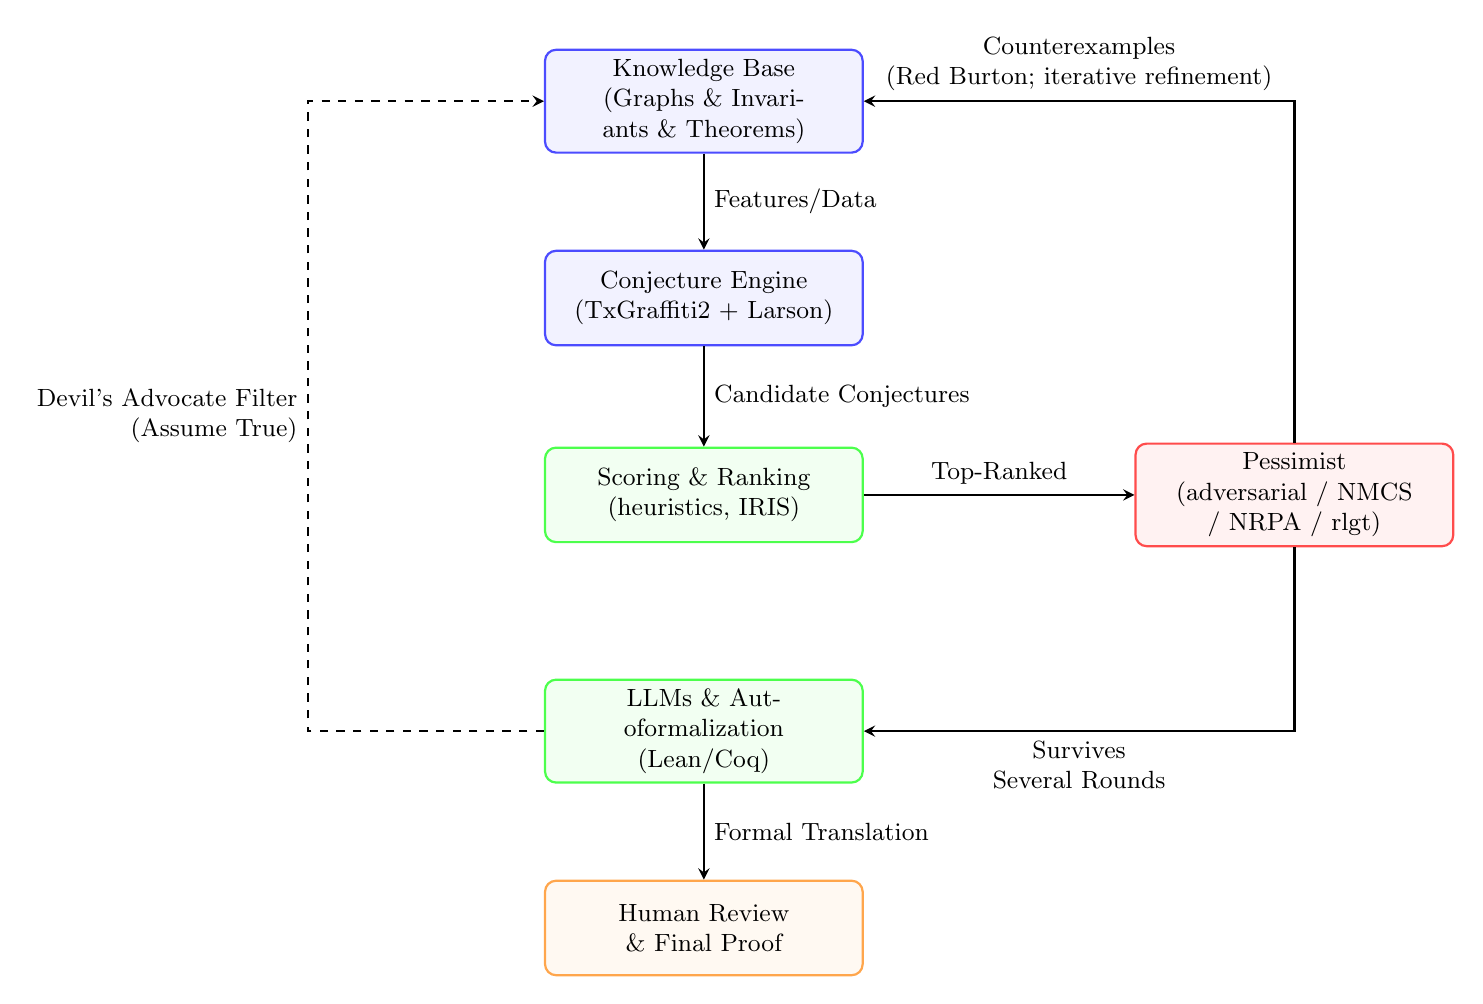
\begin{tikzpicture}[
        box/.style={draw=blue!70, fill=blue!5, rectangle, rounded corners, minimum width=3.8cm, minimum height=1.2cm, align=center, text width=3.8cm, thick},
        pessimist/.style={draw=red!70, fill=red!5, rectangle, rounded corners, minimum width=3.8cm, minimum height=1.2cm, align=center, text width=3.8cm, thick},
        extension/.style={draw=green!70, fill=green!5, rectangle, rounded corners, minimum width=3.8cm, minimum height=1.2cm, align=center, text width=3.8cm, thick},
        human/.style={draw=orange!70, fill=orange!5, rectangle, rounded corners, minimum width=3.8cm, minimum height=1.2cm, align=center, text width=3.8cm, thick},
        arrow/.style={->, thick, >=stealth},
        font=\small
    ]
    % Nodes
    \node[box] (kb) at (0, 0) {Knowledge Base \\ (Graphs \& Invariants \& Theorems)};
    \node[box] (engine) at (0, -2.5) {Conjecture Engine \\ (TxGraffiti2 + Larson)};
    \node[extension] (iris) at (0, -5) {Scoring \& Ranking \\ (heuristics, IRIS)};
    \node[pessimist] (pessimist) at (7.5, -5) {Pessimist \\ (adversarial / NMCS / NRPA / rlgt)};
    \node[extension] (autoformal) at (0, -8) {LLMs \& Autoformalization \\ (Lean/Coq)};
    \node[human] (human) at (0, -10.5) {Human Review \\ \& Final Proof};

    % Main flow arrows
    \draw[arrow] (kb) -- node[right] {Features/Data} (engine);
    \draw[arrow] (engine) -- node[right] {Candidate Conjectures} (iris);
    \draw[arrow] (iris) -- node[above] {Top-Ranked} (pessimist);

    % Loop back from Pessimist
    \draw[arrow] (pessimist.north) |- node[above, pos=0.75, align=center] {Counterexamples \\ (Red Burton; iterative refinement)} (kb.east);

    % Success path from Pessimist
    \draw[arrow] (pessimist.south) |- node[below, pos=0.75, align=center] {Survives \\ Several Rounds} (autoformal.east);

    % Autoformalization to Human
    \draw[arrow] (autoformal) -- node[right] {Formal Translation} (human);

    % Devil's Advocate Filter
    \draw[arrow, dashed] (autoformal.west) -- ++(-3,0) |- node[left, pos=0.25, align=right] {Devil's Advocate Filter \\ (Assume True)} (kb.west);
    \end{tikzpicture}}
    \caption{The integrated automated mathematical discovery pipeline.
    Conjectures are generated, immediately scored and ranked (heuristics, IRIS),
    and then aggressively tested by the refutation engine (the Pessimist:
    adversarial pool plus NMCS/NRPA/rlgt search). Only conjectures surviving
    multiple rounds of refutation are passed to LLMs for autoformalization; found
    counterexamples are minimised (Red Burton) and fed back into the knowledge
    base. The dashed line is the Devil's Advocate filter, where surviving
    conjectures are assumed true to constrain future generation, before advancing
    to final human review.}
    \label{fig:pipeline}
\end{figure}

\section{Discovery in graph theory}
\label{sec:discovery}

We now report what the pipeline actually produces on graph theory, separating a
validated search engine, exhaustive checks of open conjectures, and a frank
account of the false positives.

\subsection{A validated counterexample-search engine}
\label{sec:engine}
To attack conjectures whose counterexamples lie outside any fixed pool, we use
a structure-seeded search: a large library of parametric graphs (barbells,
double stars, lollipops, split graphs, spiders, regular graphs, $\alpha=2$
complements) is generated for each order $n$, and each seed is driven to a
local optimum of the violation margin by best-improvement edge-flip hill
climbing (with degree-preserving $2$-swaps for regular-graph targets). Plain
cross-entropy over independent edge probabilities was tried first and
\emph{failed} its validation---it could not represent the block structure of a
barbell---which is why seeding from structured graphs is essential.

The seeded engine validates on real published conjectures. For the
Aouchiche--Hansen conjecture $\lambda_1(G)+\mu(G)\ge\sqrt{n-1}+1$ (with the star
as the conjectured extremal)~\cite{aouchiche2009variable}, it independently found the optimal counterexample
at $n=18$: a subdivided double star with $\lambda_1+\mu=5.1013<\sqrt{17}+1$, a
violation margin of $0.02181$ that matches the published optimal score of an
adaptive Monte-Carlo refutation~\cite{roucairol2022refutation,roucairol2025refutation} to five decimals. It likewise refuted the
\textsc{AutoGraphiX} conjecture $\lambda_1(G)\cdot\pi(G)\le n-1$
($\pi$ proximity) at $n=11$.

\subsection{Open conjectures: exhaustive and seeded attacks}
\label{sec:open}
We then aimed the engine and the exhaustive census at open conjectures stated
exactly (from formal sources). Table~\ref{tab:open} summarises. Every
correctly-implemented open conjecture held; the falsifiable conjectures we
refuted were the ones already known to be false.

\begin{table}
  \caption{Open conjectures tested with exact statements.}
  \label{tab:open}
  \begin{tabular}{lll}
    \toprule
    Conjecture & Test & Result\\
    \midrule
    Reed $2\chi\le\omega+\Delta+2$ & search $n\le15$ & holds (tight)\\
    indep.\ dom.\ (arXiv 2107.00295) & search $n\le21$ & holds\\
    TxGraffiti $\alpha\ge\tfrac{a+R}{\Delta}$ & search $n\le28$ & holds\\
    TxGraffiti $Z\le\alpha+1$ ($\Delta\le3$) & search $n\le14$ & holds\\
    Mirror $i\le\mu^\ast$ ($r$-regular) & $2$-swap $n\le22$ & holds\\
    Graffiti.pc 58,59,61,109 & exhaustive $n\le9$ & holds\\
    Graffiti.pc 194,198a (Ham.) & exhaustive $n\le9$ & holds\\
    Graffiti.pc 2,19,103,141--146, & exhaustive $n\le8$ & holds\\
    \quad 160,200,217,291,314--322 & & \\
    \midrule
    Aouchiche--Hansen $\lambda_1+\mu$ & seeded search & \emph{refuted} (known)\\
    AGX $\lambda_1\pi\le n-1$ & seeded search & \emph{refuted} (known)\\
    \bottomrule
  \end{tabular}
\end{table}

The exhaustive checks are themselves a small contribution: six Graffiti.pc/%
TxGraffiti conjectures are now computationally confirmed on all $273{,}191$
connected graphs of order at most nine.

\subsection{The discipline of rejecting one's own discoveries}
\label{sec:integrity}
The pipeline produced several apparent ``discoveries.'' Every one was rejected
by verification; we list them because the rejections, not the candidates, are
the point. The database artefacts $\delta\le\lambda+5$ and $\chi\le 2m/n+3$ held
on the whole corpus but are false; the adversarial pool exhibits the barbell and
clique-plus-tail witnesses. The bound $n\le m+1$ ``survived'' everywhere because
it merely asserts connectivity ($m\ge n-1$), and the corpus is connected.

\section{Discussion}

Two independent expert reviews of our generated candidates, and every search
and exhaustive test we ran, reached the same conclusion: within linear and
product inequalities among classical invariants on standard graph collections,
the survivors after filtering are classical theorems, trivial structural facts,
or fitted/order artefacts. This is unsurprising given the maturity of the
field, and the pipeline rediscovering Fajtlowicz--Saks ($\mathrm{rad}\le\alpha$)~\cite{larson_survey},
Sumner--Las~Vergnas ($n\le2\nu+1$ for claw-free graphs), and the greedy and
domination product bounds is the evidence that it functions correctly, not a
disappointment. Surveys of computer-assisted graph theory~\cite{jooken2025computer} and
automated conjecture-making~\cite{larson_survey} confirm that this remains the typical experience
in mature areas. Genuine novelty in this setting requires either leaving the
inequality-fitting paradigm (structural/existential statements, program
evolution for extremal constructions, neurosymbolic reasoning~\cite{feeney2025scalar}) or matching exotic invariant definitions
exactly against formal sources---both beyond inequality search over a finite
database.

\section{Conclusion}

We built an automated graph-conjecturing pipeline whose distinguishing property
is honesty: exact-or-blank data validated against an authoritative reference; a
novelty filter that decides logical implication rather than template matching;
a permanent adversarial stage that refutes database-only artefacts and persists
its counterexamples; and a counterexample-search engine validated at the
published state of the art. The system produced no new theorem, and we resist
the temptation to manufacture one. Its durable contributions are the
methodology, the exact-or-blank combined database, the exhaustive verification
of several open conjectures up to nine vertices, and a documented discipline
that caught and dissolved every false positive. We argue that for automated
mathematics, a system that refuses to fool
itself is more valuable than one that occasionally appears to discover.

\begin{acknowledgments}
  We thank the maintainers of House of Graphs, the
  \texttt{google-deepmind/formal-conjectures} project, and the authors of
  \textsc{TxGraffiti} and \textsc{AutoGraphiX}, whose precise statements and
  data made rigorous verification possible.
\end{acknowledgments}

\section*{Declaration on Generative AI}
During the preparation of this work, the author(s) used a large language model
as a coding and experimentation assistant to implement the pipeline, run the
experiments, and draft the manuscript. All computational results were verified
against authoritative data (House of Graphs) and exact recomputation; the
author(s) reviewed and edited all content and take full responsibility for the
publication's content.

\bibliography{sample-ceur}

\appendix

\section{Reproducibility}

The methods are released as the \textsf{graphconj} package, built on
\textsc{TxGraffiti2}~\cite{davila2024automated} and
\textsc{GraphCalc}~\cite{davila2025graphcalc}, with the following layout. The
canonical invariant backend and the cross-backend honesty gate are
\texttt{invariants/graphcalc\_backend.py}, \texttt{invariants/networkx\_back\-end.py},
and \texttt{invariants/crossvalidate.py}; the exact-or-blank store and the
\textsc{TxGraffiti2} \texttt{KnowledgeTable} builder are
\texttt{data/store.py} and \texttt{data/knowledge\_table.py}, with
\texttt{data/ingest.py} ingesting the combined corpus (HoG export and the
exhaustive $n\le 9$ census). Generation, the implication-deciding novelty
filter, the Graffiti-lineage selection heuristics and IRIS scoring, and
falsification over native \textsc{TxGraffiti2} \texttt{Conjecture} objects are
\texttt{generate/txgraffiti.py}, \texttt{filter/novelty.py},
\texttt{filter/heuristics.py}, \texttt{filter/score.py},
\texttt{refute/adversarial.py}, and the interchangeable counterexample-search
backends \texttt{refute/search.py} (seeded), \texttt{refute/montecarlo.py}
(NMCS/NRPA), and \texttt{refute/rlgt.py} (cross-entropy); witnesses are
minimised by \texttt{refute/minimize.py} (Red Burton) and folded back by
\texttt{data/dynamic.py} (dynamic database). The
Larson--Van~Cleemput \textsc{Conjecturing} engine is vendored under
\texttt{sage/} (its C search core, the Sage interface, and the spec-driven
driver \texttt{run\_spec.sage}) and is invoked only across the file-spec
boundary in \texttt{generate/conjecturing\_job.py}; its expression trees are
parsed into native conjectures by \texttt{generate/expr\_bridge.py} and combined
with the coefficient-tuning linear program in \texttt{generate/tuning.py}. Each pipeline stage maps to
a SLURM batch script under \texttt{hpc/slurm/} and an Apptainer definition under
\texttt{hpc/apptainer/} (separate images for the pure-Python core and the Sage
engine), chained by \texttt{hpc/submit\_pipeline.sh}; the same subcommands
(\texttt{graphconj ingest\,|\,crossvalidate\,|\,discover\,|\,conjecture}) run
unchanged on a single machine. The honesty gate ($0$ mismatches over the shared
exact invariants) and the ingestion path are covered by the package test suite.

\end{document}
